\chapter{Instancia de Sioux-Falls}
\label{sect:siouxfallsdata}

La red de Sioux-Falls está basada en una ciudad real pero en la práctica los datos refieren a un caso abstracto y, al menos para este estudio, no es relevante conocer las unidades de los parámetros de la red.

Esta instancia se utilizó para las pruebas de validación y de sensibilidad de parámetros. Aquí se especifican los datos del grafo, costos de usuario sobre la tecnología base y de construcción de la tecnología 1 bajo el mismo valor, en la Tabla \ref{table:siouxfallsgraphdata}; y datos de demanda en Tabla \ref{table:siouxfallsdemanddata}. La representación se puede observar en la Figura \ref{fig:siouxfallsapendix}. Los datos de nodos y arcos fueron obtenidos del repositorio de instancias de redes de transporte \footnote{Transportation Networks Repository \url{https://github.com/bstabler/TransportationNetworks}}, mientras que los pares origen-destino y valores de demanda fueron tomados de \parencite{Liu2019}.

\begin{figure}[h!]
\centering
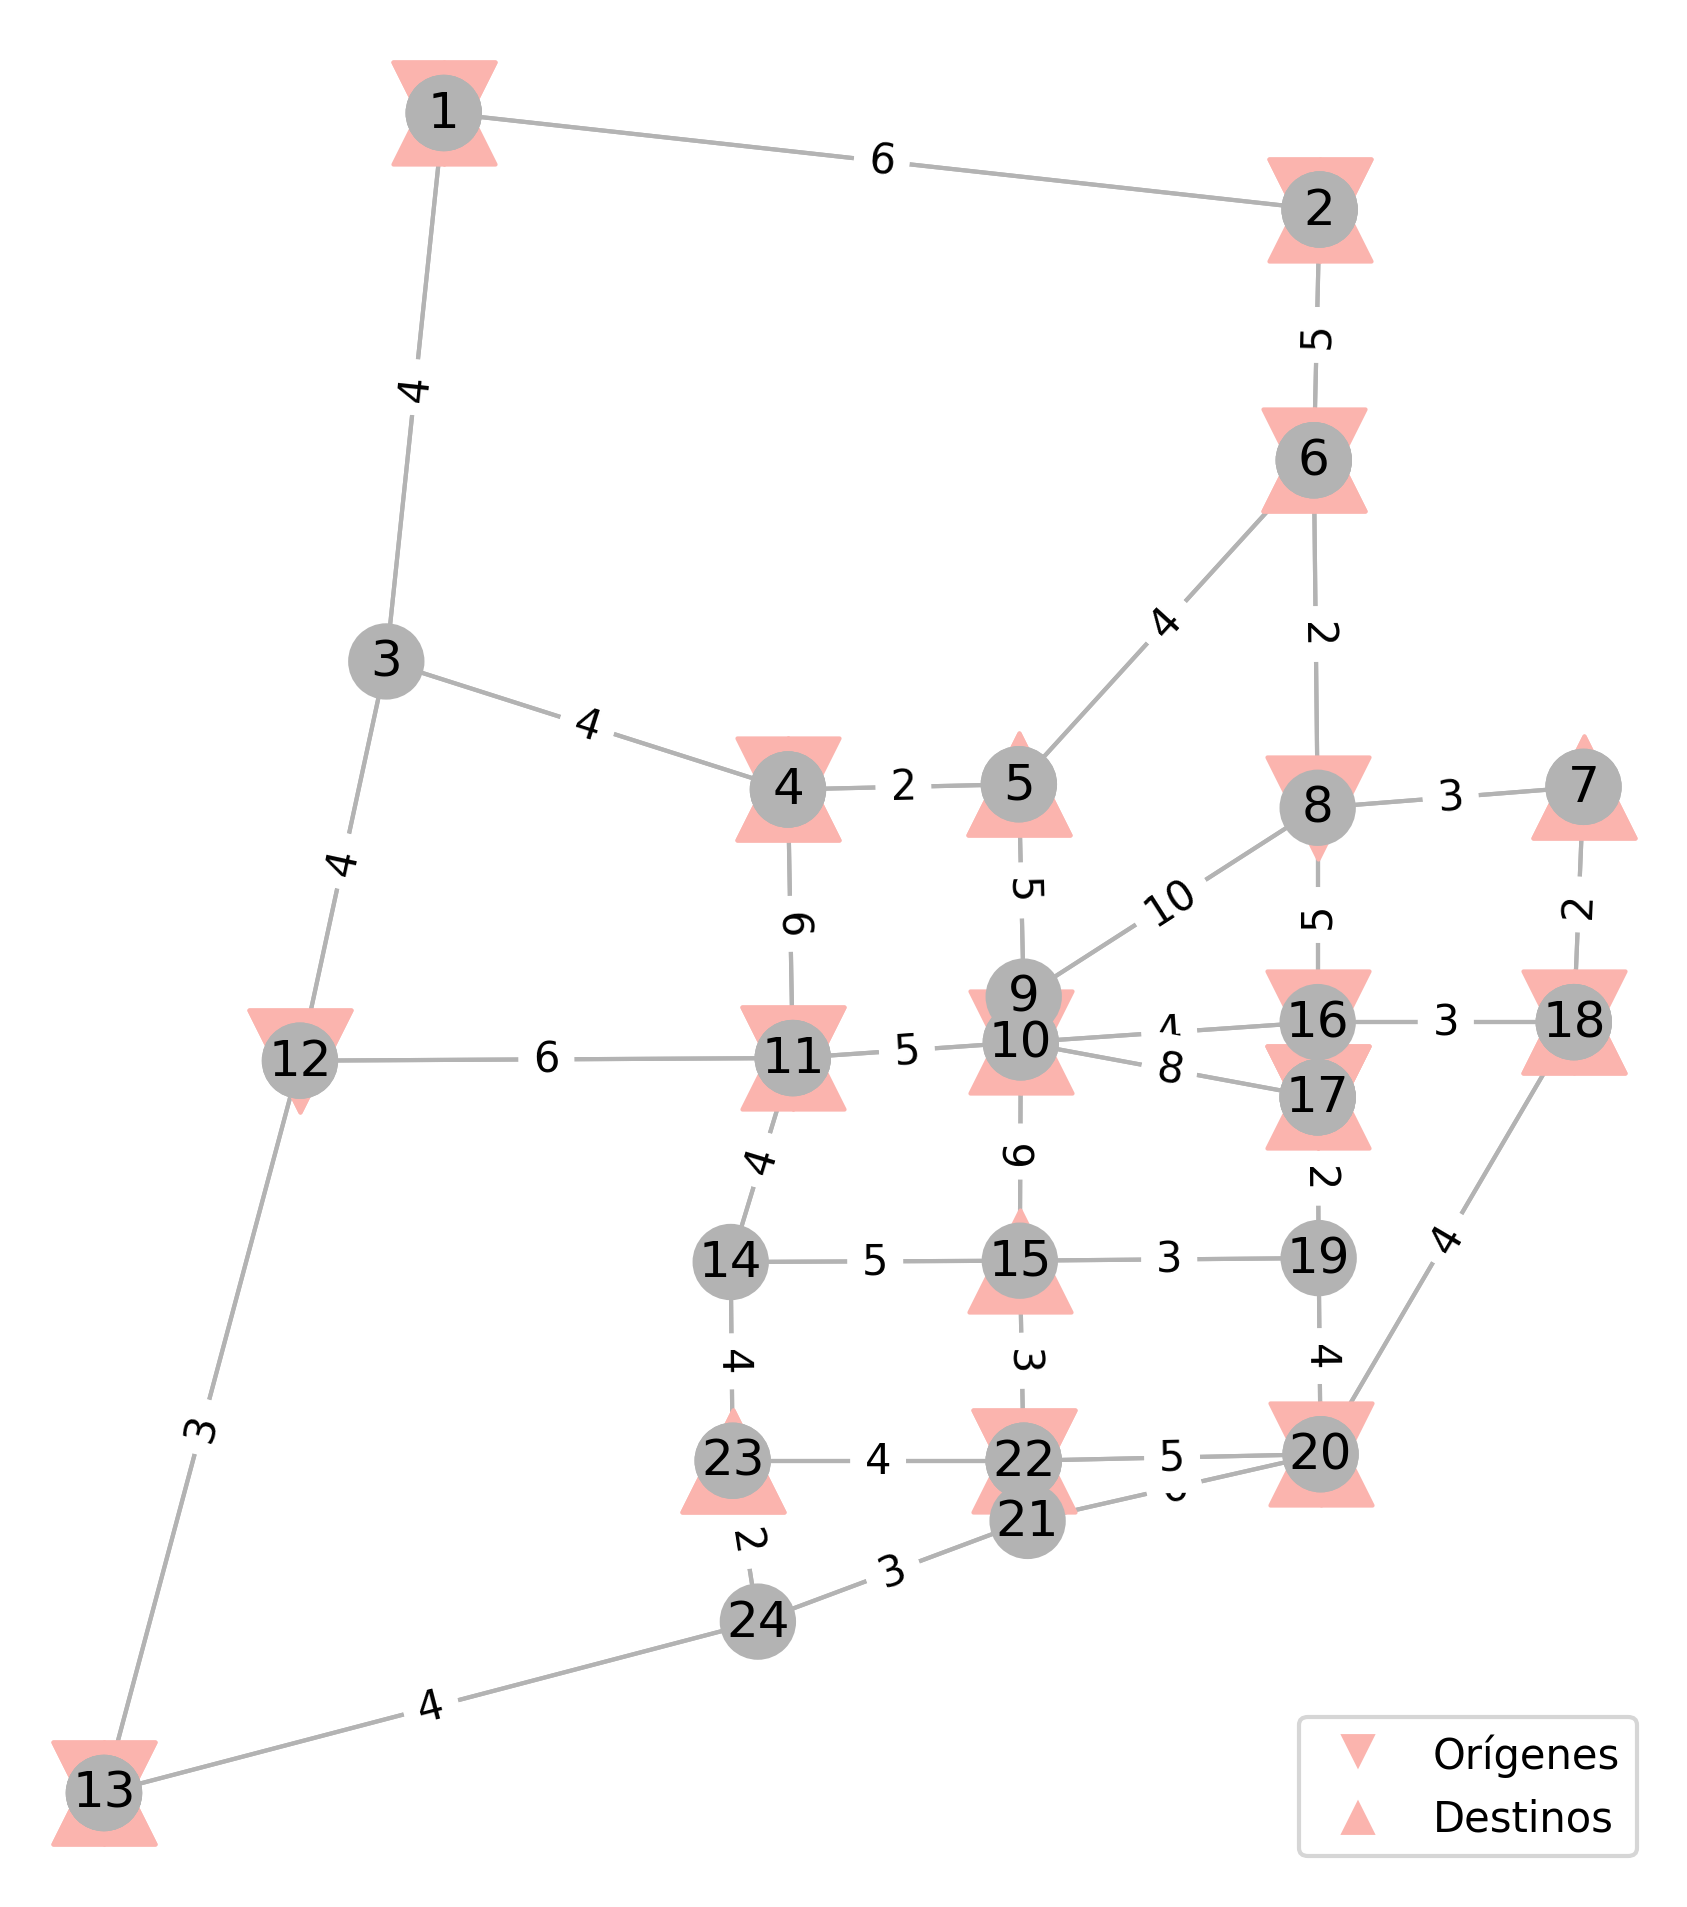
\includegraphics[width=6cm]{../resources/sioux_falls_odpairs.png}
\caption{Representación de la red de la instancia de Sioux-Falls.}
\label{fig:siouxfallsapendix}
\end{figure}

\begin{table}[h!]
\centering
\begin{tabular}{ccc}
  \toprule
    Arco & Costo \\
  \midrule
    (1, 2) & 6 \\
    (1, 3) & 4 \\
    (2, 1) & 6 \\
    (2, 6) & 5 \\
    (3, 1) & 4 \\
    (3, 4) & 4 \\
    (3, 12) & 4 \\
    (4, 3) & 4 \\
    (4, 5) & 2 \\
    (4, 11) & 6 \\
    (5, 4) & 2 \\
    (5, 6) & 4 \\
    (5, 9) & 5 \\
    (6, 2) & 5 \\
    (6, 5) & 4 \\
    (6, 8) & 2 \\
    (7, 8) & 3 \\
    (7, 18) & 2 \\
    (8, 6) & 2 \\
    (8, 7) & 3 \\
    (8, 9) & 10 \\
    (8, 16) & 5 \\
    (9, 5) & 5 \\
    (9, 8) & 10 \\
    (9, 10) & 3 \\
    (10, 9) & 3 \\
  \bottomrule
\end{tabular}
\begin{tabular}{ccc}
  \toprule
    Arco & Costo \\
  \midrule
    (10, 11) & 5 \\
    (10, 15) & 6 \\
    (10, 16) & 4 \\
    (10, 17) & 8 \\
    (11, 4) & 6 \\
    (11, 10) & 5 \\
    (11, 12) & 6 \\
    (11, 14) & 4 \\
    (12, 3) & 4 \\
    (12, 11) & 6 \\
    (12, 13) & 3 \\
    (13, 12) & 3 \\
    (13, 24) & 4 \\
    (14, 11) & 4 \\
    (14, 15) & 5 \\
    (14, 23) & 4 \\
    (15, 10) & 6 \\
    (15, 14) & 5 \\
    (15, 19) & 3 \\
    (15, 22) & 3 \\
    (16, 8) & 5 \\
    (16, 10) & 4 \\
    (16, 17) & 2 \\
    (16, 18) & 3 \\
    (17, 10) & 8 \\
    (17, 16) & 2 \\
 \bottomrule
\end{tabular}
\begin{tabular}{ccc}
  \toprule
    Arco & Costo \\
  \midrule
    (17, 19) & 2 \\
    (18, 7) & 2 \\
    (18, 16) & 3 \\
    (18, 20) & 4 \\
    (19, 15) & 3 \\
    (19, 17) & 2 \\
    (19, 20) & 4 \\
    (20, 18) & 4 \\
    (20, 19) & 4 \\
    (20, 21) & 6 \\
    (20, 22) & 5 \\
    (21, 20) & 6 \\
    (21, 22) & 2 \\
    (21, 24) & 3 \\
    (22, 15) & 3 \\
    (22, 20) & 5 \\
    (22, 21) & 2 \\
    (22, 23) & 4 \\
    (23, 14) & 4 \\
    (23, 22) & 4 \\
    (23, 24) & 2 \\
    (24, 13) & 4 \\
    (24, 21) & 3 \\
    (24, 23) & 2 \\
     & \\
     & \\
  \bottomrule
\end{tabular}
\caption{Costos de usuario de la tecnología base y de construcción de la tecnología 1 por arco de la red. Dado que utilizamos el largo del arco estos costos coinciden con dicho valor.}\label{table:siouxfallsgraphdata}
\end{table}

\begin{table}[h!]
\centering
\begin{tabular}{ccc}
  \toprule
    Origen & Destino & Demanda \\
  \midrule
    1 & 7 & 34 \\
    1 & 23 & 3 \\
    2 & 13 & 6 \\
    2 & 17 & 4 \\
    4 & 11 & 9 \\
    6 & 1 & 14 \\
    8 & 15 & 10 \\
    10 & 22 & 13 \\
    11 & 5 & 20 \\
    11 & 13 & 1 \\
    12 & 2 & 6 \\
    12 & 10 & 27 \\
    13 & 4 & 5 \\
    13 & 6 & 12 \\
    16 & 18 & 10 \\
    17 & 5 & 9 \\
    17 & 20 & 13 \\
    17 & 23 & 14 \\
    18 & 6 & 16 \\
    20 & 7 & 11 \\
    22 & 4 & 15 \\
    22 & 18 & 6 \\
  \bottomrule
\end{tabular}
\caption{Pares origen-destino utilizados para la red de Sioux-Falls junto a su valor de demanda.}\label{table:siouxfallsdemanddata}
\end{table}
